% LaTeX Template for Project Report, Version 2.0
% (Abstracted from a Major Project Report at CSED, NIT Calicut but can be
% modified easily to use for other reports also.)
%
% Released under Creative Commons Attribution license (CC-BY)
% Info: http://creativecommons.org/licenses/by/3.0/
%
%
% It is advisable to learn the basics of LaTeX before using this template.
% A good resource to start with is http://en.wikibooks.org/wiki/LaTeX/
%
% All template fields are marked with a pair of angular brackets e.g. <title here>
% except for the ones defining citation names in ref.tex.
%
% Empty space after chapter/section/subsection titles can be used to insert text.
% Just compile this file using pdflatex after making all required changes.


\documentclass[12pt,a4paper]{report}
\usepackage{listings}
\usepackage[pdftex]{graphicx} %for embedding images
\usepackage{url} %for proper url entries
\usepackage[bookmarks, colorlinks=false, pdfborder={0 0 0}, pdftitle={}, pdfauthor={Sharath Hari N, Sudev A C}, pdfsubject={Major Project Review}, pdfkeywords={Minix}]{hyperref} %for creating links in the pdf version and other additional pdf attributes, no effect on the printed document
%\usepackage[final]{pdfpages} %for embedding another pdf, remove if not required

\begin{document}
\renewcommand\bibname{References} %Renames "Bibliography" to "References" on ref page

%include other pages
\begin{titlepage}

\begin{center}

\textup{\small {\bf CS4098 Project} \\ Report}\\[0.2in]

% Title
\Large \textbf {Experimenting with Minix Operating System}\\[0.5in]

       \small \emph{Submitted in partial fulfillment of\\
        the requirements for the award of the degree of}
        \vspace{.2in}

       {\bf Bachelor of Technology \\in\\ Computer Science and Engineering}\\[0.5in]

% Submitted by
\normalsize Submitted by \\
\begin{table}[h]
\centering
\begin{tabular}{lr}\hline \\
Roll No & Names of Students \\ \\ \hline
\\
B100312CS & Sudev A C \\
B100229CS & Sharath Hari N \\ 
 \\ \hline 
\end{tabular}
\end{table}

\vspace{.1in}
Under the guidance of\\
{\textbf{Dr. K. Muralikrishnan}}\\[0.2in]

\vfill

% Bottom of the page

\includegraphics[width=0.18\textwidth]{./nitc-logo}\\[0.1in]
\Large{Department of Computer Science and Engineering}\\
\normalsize
\textsc{National Institute of Technology Calicut}\\
Calicut, Kerala, India -- 673 601 \\
\vspace{0.2cm}
Monsoon Semester 2013

\end{center}

\end{titlepage}

\newpage
\thispagestyle{empty}

\begin{center}

\huge{Department of Computer Science and Engineering}\\[0.5cm]
\normalsize
\textsc{National Institute of Technology Calicut}\\[2.0cm]

\emph{\LARGE Certificate}\\[2.5cm]
\end{center}
\normalsize This is to certify that this is a bonafide record of the project presented by the students whose names are given below during Winter semester 2014 in partial fulfilment of the requirements of the degree of Bachelor of Technology in Computer Science and Engineering.\\[1.0cm]

\begin{table}[h]
\centering
\begin{tabular}{lr}
Roll No & Names of Students \\ \\ \hline
\\
B100312CS & Sudev A C \\ 
B100229CS & Sharath Hari N \\
\end{tabular}
\end{table}

\vfill


% Bottom of the page
\begin{flushright}
Dr K. Muralikrishnan\\
(Project Guide)\\[1.5cm]
Jayaraj P B\\
(Course Coordinator)\\
\end{flushright}

\begin{flushleft}
Date: 14/05/2014
\end{flushleft}

\vspace{2in}
\begin{abstract}
This project aims to study the Minix 3 microkernel and implementing the support for immediate files which is currently unavailable.An immediate file is a file whose data is not stored in a data block, but directly inside the inode itself. With such an implementation, data fragmentation in the file system caused by small files can be solved and number of disk accesses can be reduced.

\end{abstract} 


\pagenumbering{roman} %numbering before main content starts
\tableofcontents


%\listoffigures

\newpage
\pagenumbering{arabic} %reset numbering to normal for the main content

\chapter{Problem Statement}

%Implementation of an immediate file in MINIX 3 file system, which will help in saving space and improve the %performance for small files. Files smaller than 32 Bytes can be accommodated in the inode itself which is usually %used to store the pointers to disk block. 
\vspace{10mm}

Understand the VFS and implement support for Immediate Files in Minix Filesystem.\\ \linebreak
 {\bf Specifications}:\\
\begin{itemize}
\item An Immediate file is created only when we pass an open flag O\_CREATI (you will have to define this open flag constant).
\begin{itemize}
\item by default we use open system calls to create a regular file:
    open("filename", O\_CREAT , 0666);
    
\item  now for creating immediate file we will define a new constant O\_CREATI and open system call with parameter O\_CREATI should create an immediate file:
    open("filename", O\_CREATI, 0666);   
\end{itemize}

\item All other file operations (open, delete, read, write ...) should work on immediate files.
\item When size of immediate file reaches 32 Bytes the filesystem should return an error. 

\end{itemize}


 %objective changed to problem definition
\chapter{Introduction}

\section{Literature Review}

\vspace{10mm}
 Construction of a Highly Dependable Operating System, { \em Jorrit N. Herder, Herbert Bos, Ben Gras, Philip Homburg, and Andrew S. Tanenbaum - Vrije Universiteit, De Boelelaan 1081a, 1081 HV Amsterdam, The Netherlands
}\cite{chdos}
\\
\\
This paper discusses how we can design and implement a highly dependable system { \em MINIX 3} what problems are encountered, and how they are solved. They also discuss the performance effects of the changes and evaluate how the multiserver design improves operating system dependability over monolithic designs. While the emphasis is on a more reliable operating system MINIX 3 fails to better MINIX 2 in performance. One of the changes proposed to improve performance is with the filesystem where they experimented with different block sizes.

\vspace{10mm}

Immediate files, { \em  Sape. J. Mullender and Andrew S Tannenbaum - Software practice and experience April 1984 }\cite{astimme}
\\
\\
A efficient disk organization is proposed in this paper. The idea is store the first part of data inside the inode itself instead of storing the pointers there. As per the paper about 60.87 \% of the files in unix are lesser than 2048 bytes or less which means most of the files are short. Immediate blocks can be used to reduce the no of disk access considering most files being short.

\pagebreak
How To Manipulate the Inode Structure  { \em Karthick Jayaraman, Syracuse University } \cite{inode}
\\ 
\\
The Minix filesystem is briefly explained with a note on how to manipulate and store data into the inode sturcture. Inode's internal details is explained in depth.

\vspace{10mm}

Operating Systems Design and Implementation Third Edition { \em Andrew S Tanenbaum, Albert S Woodhull }\cite{ast}
\\
\\
The operating system concepts are discussed in this book using the MINIX 3 operating system model and source code. Entire source code of MINIX 3 is available in this book. The book explains MINIX 3 filesystem in great detail. 

%\subsubsection{<Sub-subsection title>}
%even more text\footnote{<footnote here>}, and even more.

\vspace{10mm}
 Design and implementation of the MINIX Virtual File system, { \em Balazs Gerofi, August 2006 - Vrije Universiteit, The Netherlands
}\cite{vfs}
\\
\\
This paper presents a general description of the Minix Virtual File system layer.It covers the design principles, the components and their functionalities.
The various data structures used in the Virtual File System and the operations related to them are described. The communication between the VFS and the actual file system implementations are explained to a great extent.
In order to demonstrate the overall mechanism of the MINIX Virtual File system, the paper provides the main steps of the execution of a system call which gives a clear idea about the structure of the VFS.
Overall, an abstract layer has been designed and implemented, which is in charge of controlling the overall mechanism of the VFS by issuing accurate requests for the appropriate FS servers during the system calls.


\section{Minix}



Instead fo reading this introduction it will be better if you watch Andrew Tanenbaums talk on Minix 3 given at FOSDEM.

Different kinds of people use computers now than sev­eral decades ago, but operating systems have not fully kept pace with this change. Early users expected the computer to crash often; reboots came as naturally as waiting for the neighborhood TV re­pairman to come replace the picture tube on their home TVs. All that has changed and operating systems need to change with the times.Modern computer users are from a broad cross-section of society. Most of them have a set of mental expectations that we call The TV model.
It goes like this:
\begin{itemize}
\item You buy the device.
\item You turn it on.
\item It works perfectly for the next 10 years.
\end{itemize}

Most electronic devices fit this model well, the one exception being the personal computer. In addition to mind-numbing complexity (e.g., even networking experts have trouble configuring a wireless base station, despite the 500-page manual), they are prone to crashes and blue screens of death, issues unheard of with other electronic devices.

Most modern computer users want their systems to work all the time and never crash, ever. In engineering terms, this requires a mean time to failure (MTTF) appre­ciably longer than the expected lifetime of the computer.The average user virtually never complains that the com­puter itself is too slow (e.g., it cannot update a spread­sheet fast enough), although complaints about the speed of the Web are common. Over time, the relationship be­tween speed and reliability has reversed. Most users now consider the reliability of the computer to be far more im­portant than its speed, the reverse of 40 years ago.

Yet operating system reliability is still poor. To make the research challenge more explicit, consider a device driver that contains a fatal bug such as a store through an invalid pointer or an infinite loop. In commodity op­erating systems, when this bug is triggered, it crashes or hangs the entire system because the buggy code is run­ning in kernel mode. All user programs that were run­ning at the time the bug struck are killed, all user work is lost, and all FTP, Web, and e-mail transfers are abruptly aborted.

Studies have shown that software contains about 6-16 bugs per 1000 lines of code, it is simply infeasible to get all code to be correct. Therefore, the MINIX OS was designed in such a way that certain major faults are properly isolated, defects are detected, and failing components can be replaced on the fly, often transparent to applications and without user intervention or loss of data or work.  

\subsection{MINIX 3 and its architecture}

MINIX 3 is a microkernel based POSIX compliant operating system designed to be highly reliable, flexible, and secure. The approach is based on the ideas of modularity and fault isolation by breaking the system into many self-contained modules. In general the MINIX design is guided by the following principles:

\begin{itemize}
\item Simplicity: Keep the system as simple as possible so that it is easy to understand and thus more likely to be correct.

\item Modularity: Split the system into a collection of small, independent modules and therefore prevent failures in one module from indirectly affecting another module.

\item Least authorization: Reduce privileges of all modules as far as it is possible.

\item Fault tolerance: Design the system in a way that it withstands failures. Detect the faulty component and replace it, while the system continues running the entire time.
\end{itemize}

The operating system is structured as follows. A minimal kernel provides interrupt handlers, a mechanism for starting and stopping processes, a scheduler, and interprocess communication. Standard operating system functionality that is usually present in a monolithic kernel is moved to user space, and no longer runs at the highest privilege level. Device drivers, the file system, the network server and high-level memory management run as separate user processes that are encapsulated in their private address space.

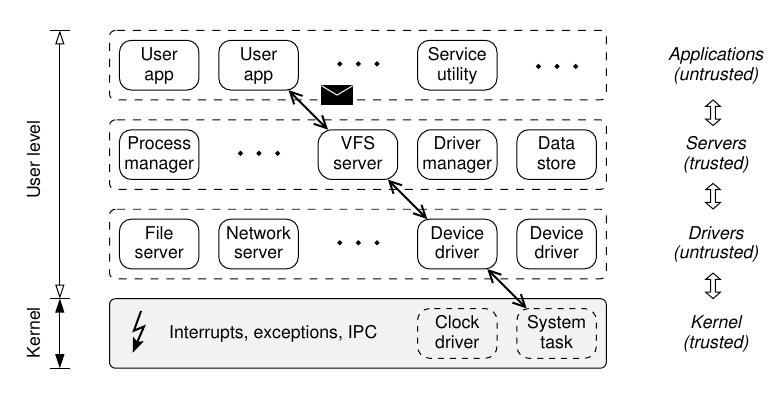
\includegraphics[scale=0.7]{./pics/minixarch.png}

The above figure shows the structure of the operating system.\\

Although from the kernel’s point of view the server and driver processes are also just user-mode processes, logically they can be structured into three layers. The lowest level of user-mode processes are the device drivers, each one controlling some device. Drivers for IDE, floppy, and RAM disks, etc. Above the driver layer are the server processes. These include the VFS server, underlying file system implementations, process server, reincarnation server, and others. On top of the servers come the ordinary user processes including shells, compilers, utilities, and application programs.\\

Because the default mode of interprocess communication (IPC) are synchronous calls, deadlocks can occur when two or more processes simultaneously try to communicate and all processes are blocked waiting for one another. Therefore, a deadlock avoidance protocol has been carefully devised that prescribes a partial, top-down message ordering. The message ordering roughly follows the layering that is described above. Deadlock detection is also implemented in the kernel. If a process unexpectedly were to cause a deadlock, the offending is denied and an error message is returned to the caller. \\

Recovering from failures is an important reliability feature in MINIX. Servers and drivers are started and guarded by a system process called the reincarnation server. If a guarded process unexpectedly exits or crashes this is immediately detected – because the process server notifies the reincarnation server whenever a server or driver terminates – and the process is automatically restarted. Furthermore, the reincarnation server periodically polls all servers and drivers for their status. If one does not respond correctly within a specified time interval, the reincarnation server kills and restarts the misbehaving server or driver.

\section{Virtual File System in MINIX 3}

Virtual File System is an abstraction layer – over the file system implementations – in the operating system. It provides a common interface for the applications so that they can access different types of underlying file systems in a uniform way and therefore the differences in their properties are hidden. This interface consist of the file system related system calls.\\

The VFS also provides a common interface for the underlying file systems and manages resources that are independent from the underlying file systems. This common interface ensures that new file system implementations can be added easily.

\subsection{VFS Design }
Exploiting modularity is a key idea behind MINIX, therefore the design of the Virtual File system layer is also driven by this idea. In contrast to the monolithic kernels, where the VFS layer access the implementation of the underlying file systems through function pointers, in MINIX the drivers are different processes and they communicate through IPC. During the design of the MINIX Virtual File system the most important decisions that had to be made were the followings:
\begin{itemize}
\item Which components are responsible for which functionalities.

\item Which resources are handled by the VFS and which are handled by the actual file system implementations.

\item  Where to divide the former FS process in order to get an abstract virtual layer and the actual MINIX file system implementation.
\end{itemize}

Comparing the MINIX VFS to the VFS layer in other monolithic UNIX kernels some functionalities have to be handled in a different way. In monolithic kernels the communication between the VFS layer and the underlying file system implementation is cheap, simple function calls, while sending messages between processes is more expensive. For this reason, keeping the number of messages low during a system call is important.

The MINIX Virtual File system is built in a distributed, multiserver, manner. It consists of a top-level VFS process and separate FS process for each mounted partition.

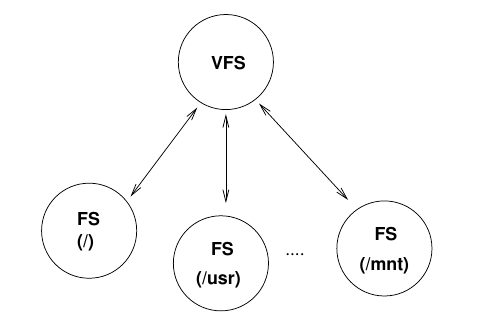
\includegraphics[scale=0.7]{./pics/vfsfs.png}

The top-level VFS process receives the requests from user programs through system calls. If actual file system operation is involved the VFS requests the corresponding FS process to do the job. This dependency is depicted in figure above. In other words all the file system calls will have to go through the virtualiztion layer first then the VFS will route it to specific file system server.

\subsection{Major steps in execution of system call}

Let's consider system call {\em stat()} with an argument {\em /usr/web/index.html} . This will help you in understanding VFS and its workflow.\\

Assume
\begin{itemize}
\item a ext2 partition mounted at /usr
\item root filesystem is Minix filesystem
\end{itemize}

\textbf{Steps}

\begin{enumerate}

\item The user process calls the stat() function of the POSIX library which builds the stat request message and sends it to the VFS process.
    (a) The VFS process copies the path name from userspace.

\item The VFS first issues a lookup for the path name. It determines that the given path is absolute, therefore the root FS process has to be requested to perform the lookup.
    (b) The root FS process copies the path name from the VFS’ address space.

\item During the lookup in the root FS process the root directory has to be read in order to find the string ”usr”. Let us assume that this information is not in the buffer cache. The root FS asks the Driver process to read the corresponding block from the disk.

\item The driver reads the block and transfers back to the FS process. It reports OK.
    (c) The driver copies the disk content into the FS’ buffer cache.

\item The root FS process examines the ”usr” directories inode data and realizes that there is a partition mounted on this directory. It sends the EENTER MOUNT message to the VFS that also contains the number of characters that were processed during the lookup.

\item The VFS looks up in the virtual mount table which FS process is responsible for the ”/usr” partition. The lookup has to be continued in that FS process ( "/usr" Mininx filesystem partition). The VFS sends the lookup request and with the rest of the path name.
    d. The ”/usr” FS process copies the path name from the VFS’ address space.

\item The FS process that handles the ”/usr” partition continues the lookup of the path name. It needs additional information from the disk, therefore it asks the driver process to read the given block and transfer it into the FS process buffer cache.

\item The driver reads the disk and transfers back to the FS process. It reports success.
    (e) The driver copies the disk content into the ”/usr” FS process’ buffer cache.

\item The "/usr" FS process finishes the lookup and transfers back the inode’s details to the VFS.

\item The VFS has all the necessary information in order to issue the actual REQ STAT request. The FS process is asked to perform the stat() operation.

\item The FS process fills in the stat buffer. Let us assume that all the information needed for this operation is in the FS process’ buffer cache, therefore no interaction is involved with the Driver process. The FS copies back to the user process’ address space. It reports success for the VFS.
    (f) The FS process copies the stat buffer to the caller process’ address space.

\item The VFS receives the response message from the FS process and sends the return value back to the POSIX library. The function reports success back to the user process.

\end{enumerate}
    
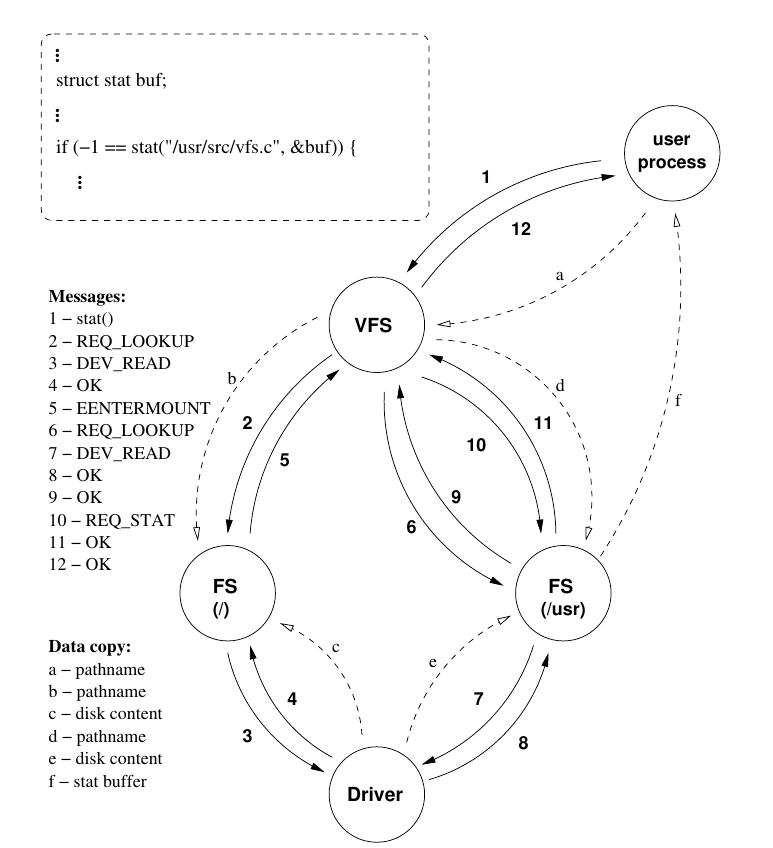
\includegraphics[scale=0.7]{./pics/vfsflow.png}

\subsection{Comparison}
Monolithic kernels are finely tuned and optimized to be efficient. Performance is one of the key issue. In contrast, the MINIX design is about reliability and security. An immediate consequence of these is that the MINIX VFS has a different structure, it has different properties. Some of these differences are given in this section.\\

As we mentioned before, kernel data structures can be easily accessed in monolithic kernels and the communication between components are simple function calls. This implies that the border between the virtual layer and the actual file system implementations is not at the same place where it is in the MINIX VFS. Monolithic kernels keep as much functionality in the VFS layer as they can.\\

Communication is free between the VFS and the underlying file system drivers therefore it makes sense to keep the virtual layer as abstract as it is possible and to reduce the functionality of the actual file system implementations. This make the implementations of a new file system easier. 

\subsection{Conclusion}

Implementation of VFS in Minix helps in creation of Virtualization layer between the kernel and other file system servers. Now implementation of any new filesystem in Minix is much easier as we don't have to deal with any other interface other than VFS and FS interface.
 %literature survey included in this
\chapter{Work Done}

\section{Setting up Minix 3 development environment}
Installation of Minix 3 was done using Virtualbox({\em Virtualization software}) in Linux based host machine.\\
%Please refer to Appendix I for detailed steps.
\section{Modification of Kernel}
\subsection{Motive}
A small project was done to familiarise with the Minix 3 operating system code base.
\subsection{Problem Statement}
Print out the name of every file that is being executed by the OS.
\subsection{Approach}
Locate the kernel source file that implements the exec system call.\\	
Insert a printf statement appropriately in the located file.\\
Rebuild the entire system.
\subsection{Solution}
The implementation of the exec system call was found in file do\_exec.c under /usr/src/kernel/system/ of the minix source tree.\\
The name of the process that is being executed is captured using the variable { \em name} and is printed out.\\
The system is rebuilt using the command {\em make clean} and { \em make build} inside /usr/src/ folder. 




\chapter{Technical Issues}

\section{Selecting the version} 

A lot of confusion preceded on which version of MINIX to work on. If it was to implement immediate files, it will be much easier to implement immediate files in MINIX 3.1(book version) which does not have VFS. With the inclusion of VFS and more functionalities, the complexity of the code increased tremendously from 3.1 to 3.2.1. If the aim was only to implement immediate files , the advise would be to go with MINIX 3.1.

\section{Installation and Networking}

\begin{itemize}
\item A considerable amount of time was spent on the installation and setting up of MINIX 3 development environment 
\item Qemu crashes during Minix installation proccess. A suspected bug was reported on Qemu crashes while installing MINIX 3 \cite{•}.
\item The installation worked well in Virtual Box, but the setting up part was a bit tricky. Openssh server was installed for the networking between the host OS and the virtual machine. We were unsuccessful due to the restrictions in the college firewall for FTP packets. We will have to open FTP ports in order to download software packages from Minix software repositories.
\end{itemize}
 

\section{Documentation Issues}

Working with the existing code is tedious when code is not documented properly. There was little documentation or support for newbies. Satisfying replies from the mailing list or the MINIX groups was newer there for newbies. The  Balazs Gerofi's Master's Thesis is only documentation in regard to VFS implementation \cite{vfs}.

%\chapter{Work Remaining}

Implement immediate files in MINIX 3 by making changes in the kernel code. An immediate file should be created by the operating system whenever a special option flag is passed to {\em creat/open } system call. The operating system should also report an error whenever the file exceeds 32 Bytes in size. A file created as an immediate file is always an immediate file and is never converted to a regular file.

\section{Inode Structure}
Below shown is the inode structure in Minix 3.

\lstinputlisting{inode.h}

The pointers to the disk block is saved in an array i\_zone each referencing a 32 bit address in the disk.This array can be used to store data when file size is lesser than 32 Bytes. 

\section{Differentiating between an immediate and regular file}

Minix file system uses the flag bits in the {\em const.h} header file for { \em i\_mode} variable of inode structure, so now we have to add flag bits to check for immediate files.

\section{Operations on an immediate file}
\subsection{Create}
Create a immediate file only when the flag bit for immediate file is set. This flag must be passed to creat/open system call.
\subsection{Read}
Instead of reading the data from the disk block the read system call should be modified to read data from the inode itself.
\subsection{Write}
The write system call should be modified to write data into the inode itself and should report an error whenever the file size goes beyond 32 Bytes.
\subsection{Delete}
When files are deleted typically indirect disk blocks need to be freed skip this step in case of immediate file and delete the inode.

\chapter{Conclusion}

A critical study of the MINIX 3 Virtual File System was done and the results of the study are summarized here. The MINIX Virtual File system is built in a distributed, multiserver manner, which is a substantially different architecture compared to other UNIX-like solutions. An abstract layer has been designed and implemented, which is in charge of controlling the overall mechanism of the VFS by issuing accurate requests for the appropriate FS servers during the system calls.It is also in charge of maintaining abstract data structures that are independent from the underlying file system drivers and are playing important roles within the Virtual File system’s functionality. In order to achieve this, several data structures and functions operating on them had to be designed and added to the former FS server. The communication with underlying file system drivers also had to be implemented. The MFS implementation had to be separated from the original code and some part of it was rewritten to cooperate with the Virtual Layer. The communication according to the VFS/FS interface also had to be implemented.\\
\\
Second part of the project was implementing support for immediate files in MINIX 3 File System. A proper design for its implementation was framed and documented in the previous chapters. Although the implementation was not complete, the process was helpful in understanding the MFS and VFS. It would have been much easier to implement support for immediate file if we make a slight change in the problem statement. We can consider all newly created files as immediate files and instead of reporting an error when the file exceeds capacity of immediate file we can actually convert them to regular files at that particular point.  


%\cleardoublepage
%\pagebreak
\phantomsection
\addcontentsline{toc}{chapter}{Acknowledgements}
\chapter*{Acknowledgments}
\vspace{1.0in}
<Acknowledgements here>
\\
\\
\\ 
\\
<Name here> \\ 
\\
<Month and Year here>\\
{National Institute of Technology Calicut}\\
\newpage

\cleardoublepage
%\pagebreak
\phantomsection
\addcontentsline{toc}{chapter}{References}
\begin{thebibliography}{99}

\bibitem{vfs} MINIX VFS {\em Balazs Gerofi, Vrije Universiteit Amsterdam } \\ \url {http://www.minix3.org/doc/gerofi_thesis.pdf}

\bibitem{astimme}Immediate Files {\em Sape. J. Mullender and Andrew S Tannenbaum - Software practice and experience April 1984 } \\  \url{http://onlinelibrary.wiley.com/doi/10.1002/spe.4380140407/abstract}


\bibitem{mbook} Operating System Design and Implementation, Third Edition{ \em Andrew S Tanenbaum, Albert S Woodhull }
\bibitem{login2010} Minix 3: status report and current research { \em ;login: JUNE 2010 } \\ \url{http://www.minix3.org/docs/login-2010.pdf}


\end{thebibliography}

\chapter{Appendix}

\section{Message Passing in MINIX}

\subsection{Message Passing Properties}

\begin{itemize}

\item Minix uses the concept of a message to support communication between processes. This is used universally througout Minix whenever one process needs to access another.

\item    Minix user processes can only send/receive messages to system processes, not to other user processes.

\item    Minix system processes can send messages to other system processes and reply to user process messages subject to certain restrictions.

\item    The following message passing functions are implemented by the kernel:
	\begin{itemize}
	  \item   send
      \item   receive
      \item   sendrec (send/receive)
      \item   notify
      \item   echo
	\end{itemize}
       

\item The first three use the rendezvous style message passing. So sendrec in a user process will block the user if the destination system process is currently doing something other than trying to receive an new request message.

\item The \_syscall function used by user level programs actually uses the sendrec (send/receive) function to send a request and receive a reply.

\item  The notify type message does not use the rendezvous. That is, it does not get blocked if the destination is not yet ready to receive the notification.

\item The echo is used by the kernel process for passing a message from a process to itself.

\end{itemize}

\subsection{Message Format}

A message consists of: the process ID of the sending process, an identifier telling the process what sort of message it is, and then a union for holding the actual message structure. The code snippet from the file  \emph{/usr/src/include/minix/ipc.h} shows the message structure :
\begin{small}
\lstinputlisting{./codeblocks/messagestructure}
\end{small}



MINIX 3 has 10 message types (mess\_1 to mess\_10) as we can see from the message structure above. Each of these message types are unique. The code below from the same file shows the different message types :
\begin{small}
\lstinputlisting{./codeblocks/messagetypes}
\end{small}





\end{document}
